%!TEX root = ../main.tex
%=========================================================

\section{Overview}
\label{sec:overview}

The end-goal of service discovery is for nodes to be \textit{securely discovered} under topics which they choose to be associated with. Because malicious nodes are difficult to identify in a decentralised setting, our overarching design principle is to diversify the sources of information in all the operations, specifically in registration and search. This means selection of peers with sufficient variety (in terms of their network- and application-level identifiers) during registrations and collection of search results. In the following, we provide an overview of the design and the objectives of \textit{i)} search and register operations at a single registrar, followed by \textit{ii)} the process of distributing ads and performing search across multiple registrars in the network. \Cref{tab:objectives} provides a comprehensive list of the design objectives, which we refer to in the text below.

%As a decentralised, permissionless system, anyone can freely participate in service discovery system at no cost other than running the protocol and storing a limited number of other nodes' records. This leads to some potential security issues that must be considered when designing the system. Even worse, a single malicious entity can spawn many Sybil identities that individually enter the system. Because such nodes are difficult to identify, our overarching design principle is to diversify the sources of information in all the operations, specifically in registration and search. This means selection of peers with sufficient variety (in terms of their network- and application-level identifiers) during registrations and collection of search results. \michal{It's probably better explained in the thread model}

\subsection{Registration and lookup with a registrar}

Every registrar holds a \emph{topic table}, where it stores incoming ads from advertisers, indexing by their topics. Because a topic table is a limited resource shared by multiple advertisers, it is critical to prevent misuse of the table---\eg advertisers spamming a target registrar with ad registration requests for random, bogus topics to fill up the registrar's topic table. %or make excessive ad registration requests to many registrars in an attempt to make the advertisers' topic more visible than others.

Once stored in a topic table, an ad has a limited lifetime and removed from the table upon expiration of its lifetime. While expiration allows new ads to be continuously introduced into the topic tables, spammers can still continuously place new ads at no cost. A well-known solution to such misuse is to make consumption of topic table resources costly for the advertisers, for instance, by incorporating a Proof-of-Work (PoW) puzzle scheme \hl{[]} into the registration process---\eg registrars requiring advertisers to present PoW (\ie solution) before they are allowed to place their ads. However, PoW schemes unnecessarily consume resources, promote pooling of resources to create centralised hubs, and unfairly give advantage to resource-rich nodes ~\cite{gervais2014bitcoin}. 

%\onur{are there better arguments against PoW schemes? \michal{Creates an "arms race", doesn't really solve the problem (there are papers showing that PoW blockchains are centralized with a lot of miners in China), can't run it on contraint devices. \onur{But in this case there wouldn't be a monetary reward to solve the PoW, so I am not sure if the arguments against PoW Blockchains apply to the use-case of ad registration using a PoW scheme.}}}

%At the same time, it is desirable for the ad registration process to complete in a timely manner and have as little overhead (in terms of both messaging and computation) as possible for both the registrars and advertisers. 

Instead of a PoW scheme, we propose a lightweight, \textit{waiting-time-based admission mechanism} whereby registrars enforce a waiting time on the advertisers before their ads are admitted to the topic table. Imposing this waiting time prevents misuse of the topic table, because any topic must be important enough to outweigh the cost of waiting for the advertisers, and registrars can control the rate of ad placement. 

In addition to misuse of topic table, securing topic tables from being dominantly occupied by the ads from malicious nodes (and their Sybils) is another important objective (G8). Our admission mechanism tackles this challenges through diversification of advertisers that simultaneously place ads: advertisers that contribute poorly to the diversity (in terms of their IP addresses and IDs) of the advertisers that currently have an ad in the topic table are forced to wait longer. Also, the waiting time mechanism must prevent the storage space from overflowing while aiming for \textit{a max-min fair allocation} across different topics (G1). The latter is necessary to avoid starving (unpopular) topics. %Finally, the waiting time mechanism must ensure that no advertiser is indefinitely denied from registering its ad (G1). 

%\michal{It's seems a bit redundant to the paragraph before.}
%\michal{It might be a good idea to signal already here that the waiting times is based on occupancy (cope with load) and diversity (cope with attacks + max-min fairness.}

Central to our admission mechanism is a \textit{waiting time function} that generates advertiser-specific, non-negative waiting time values. Registrars compute and return a waiting time in response to a registration request, and an advertiser receiving a waiting time must wait for the duration of the waiting time before sending a follow-up registration request to try registering with the same registrar again. For this scheme to work, registrars must be able to verify that advertisers comply with the waiting times and not serve those who try to cheat by following up early. 

Being able to check whether advertisers comply with the waiting times with as little overhead as possible is necessary to realise a lightweight registration process (G5).  
An obvious but high-overhead solution is for registrars to maintain state for each on-going registration. % which would make registrars vulnerable to state exhaustion attacks. 
Instead, we use a lightweight, \textit{token-based} mechanism whereby registrars respond to registration requests with secured, immutable tokens, \ie \textit{tickets}, containing advertiser-specific registration state including the latest computed waiting time for the advertiser. This way the burden of keeping the registration state and keeping track of when to follow up with new requests falls on the advertisers. On the other hand, the registrars' task is to simply authenticate each ticket, check if the requests comply with the waiting times, and use the state information within the tickets to compute a new waiting time.  

%In order to verify that advertisers comply with the waiting time mechanism without maintaining (per-advertiser) on-going registration state at the registrars, we propose a lightweight, \textit{token-based} mechanism whereby registrars respond to registration requests with secured, immutable tokens, \ie \textit{tickets}, containing the advertiser-specific registration state including the latest waiting time. This way the burden of keeping the registration state and keeping track of the right time to follow up falls on the advertisers. On the other hand, the registrars' task is to simply authenticate each ticket, check if the requests arrive after the tickets' waiting time has elapsed, and use the state information within the tickets to compute a new waiting time.  

%\michal{We might explicitely state that we don't create any state at the registrar but provide integrity with signatures. I'm just not sure it's not too technical for the overview.}

Once an initial ticket is obtained from the first ticket request, an advertiser must present its ticket in all the follow-up requests. Only if the new waiting time is zero, the registration is successful (\ie advertiser's ad is immediately stored in the topic table), in which case the registrar sends a confirmation of registration back to the advertiser; otherwise, the advertiser receives an updated ticket with a new waiting time. The resulting registration process is shown in Figure~\Cref{fig:registration}, where an advertiser sends a registration request, providing its ID and a desired topic (eth). Based on considerations such as the diversity of the advertiser with respect to the advertisers who currently have a ``live'' (\ie unexpired) ad and occupancy of the registrar's topic table, the registrar computes a waiting time and returns a ticket. Then, the advertiser follows up with a new request immediately after the waiting time elapses, and this time the registrar accepts the registration and places the advertiser's ad in the topic table as shown in Figure~\Cref{fig:registration}.

There are several intricacies in the design of the waiting time mechanism. For instance, the mechanism should not allow indefinite use or re-use of a ticket. Also, the mechanism should disincentivise advertisers from constantly spamming registrars with initial registration requests (without a ticket) in the hopes that they get a better waiting time, which is necessary to limit the messaging overhead of registrations (G5). We discuss these and other details in Section~\Cref{sec:waitingTime}. 

On the other hand, the search operations do not require a ticket. Once a registrar receives a lookup request for a topic from a searcher, the registrar returns a random subset of the advertisers that currently have a live ad under that topic. We discuss search and registration across multiple registrars next.

%Each time an advertiser comes back and receives a new waiting time, the registrar updates the accumulated waiting time of the advertiser as part of the  
%Otherwise, instead of a new  ticket with a positive waiting time.  follow-up request may result with a new, non-zero waiting time In this mechanism, advertisers can be repeatedly handed new tickets with each follow-up request if the waiting time function determines that the advertiser has not waited long enough. As an advertiser repeatedly receives new tickets, the registrar updates the accumulated waiting time of the advertiser in the new ticket. The accumulated waiting time is used in the waiting time function and the advertisers that accumulated longer waiting times have higher chance of placing their ads in their subsequent requests, and this guarantees that each advertiser eventually succeeds in placing its ad (G1). 

%The resulting admission mechanism is shown in \Cref{fig:registration}. An advertiser sends a registration request, providing its ID, IP address and a desired topic (eth).\michal{We should make sure that wqe used "eth" before an explained it means Ethereum mainnet. It can probably be in the intro already as one of examples.} Initially, the waiting time function computes and returns a waiting time inside a ticket. Then, the advertiser follows up with a new request once the waiting time has elapsed. In the second time, the waiting time function returns a zero waiting time, which means the advertiser's ad is placed. Finally, the advertiser receives a confirmation of registration as shown in the bottom of \Cref{fig:registration}. 

% avoid golden tickets
%There are several intricacies in the design of the waiting time mechanism. For instance, an advertiser should not be able to use a ticket indefinitely and also should not be able to re-use a ticket to register more than one ad. For this reason, tickets are only valid within a ``registration window'' which begins after the ticket's waiting time expires and ends after a short time interval of few seconds as shown in Figure ~\Cref{fig:ticket_validity}. During this interval, the registrar allows only one registration by the ticket. 

%Another important design detail is the amount of state required to enforce waiting times. We design tickets to be immutable objects that can be authenticated by the registrars. This allows registrars to avoid per-advertiser state when enforcing the waiting times---the state of a registration process is stored in a ticket, including the accumulated waiting time spent by the advertiser so far. This way the burden of keeping the registration state and acting on the waiting times is on the advertisers. 
%\michal{ok, so you actually mention state at the registrar, but later on :) Maybe bring together? Not yet sure about that. }

%One final, but important detail in the waiting time mechanism design is to avoid advertisers periodically initiating registration requests at the same registrar in the hopes that they receive a ticket with a better waiting time than the previous ones (or ideally have their ad admitted immediately). Our design ensures that searchers do not obtain better waiting times by spamming requests at a registrar and we achieve this with very little amount of state. Also, advertisers attempting to re-register an ad on a registrar that already has that ad live in its table are rejected. We discuss the details of the waiting time in Section \Cref{sec:waitingTime}.
%\michal{Might be too detailed for the overview.}

\begin{figure}
    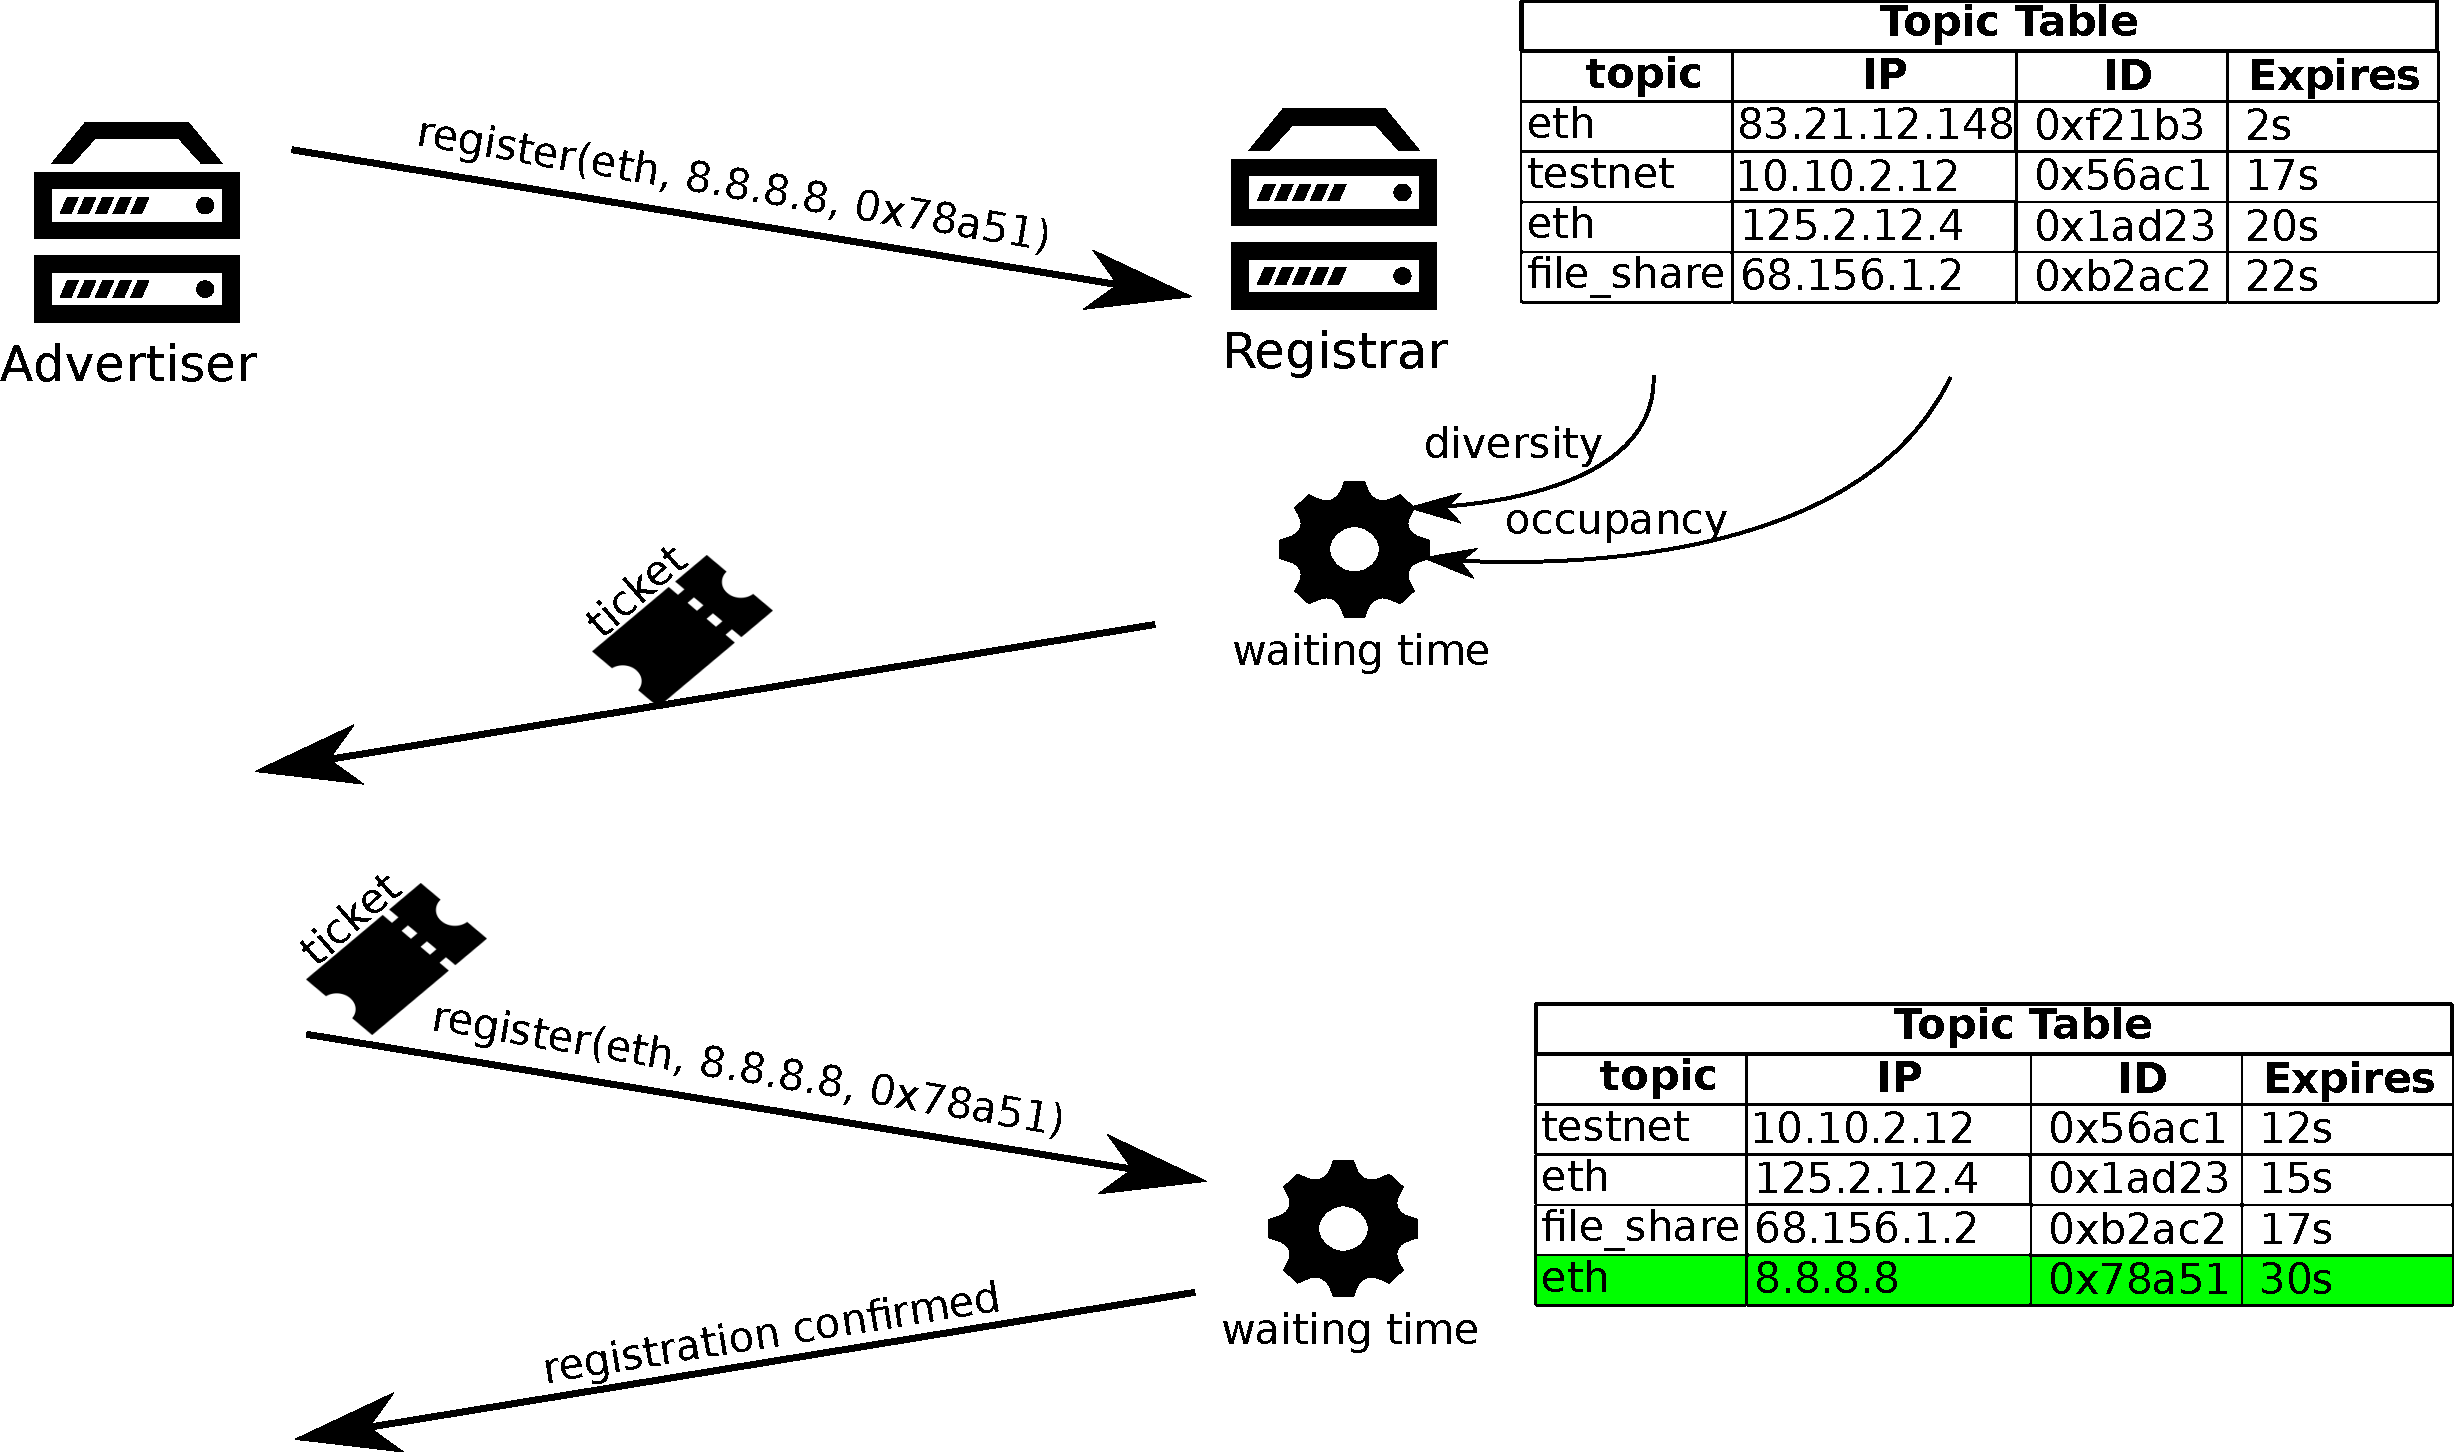
\includegraphics[width=0.5\textwidth]{img/registration}
    \caption{Registration process within one registrar.}
    \label{fig:registration}
\end{figure}


\subsection{Distributed search and registration}

In order to be discovered in the shortest time possible, advertisers are incentivised to distribute and maintain live ads across many registrars. Ideally, the topic search should be fast even for unpopular topics, \ie when the number of advertisers for a topic is much smaller than the number of all live nodes (G6). 
Given that in a decentralised setting, advertisers and registrars can not a priori agree on a subset of nodes to serve as the advertisement media for their topics, nodes must somehow find the ``right'' set of nodes at which advertisements are registered and topic lookups are sent so that they quickly meet at common nodes. While the discovery should be efficient for even the most unpopular topics (G6), the overhead of registration must ideally be equally distributed among the registrars (G3).

The main issues for the advertisers are i) on which nodes to place ads and ii) how many ads to place. For the latter issue, advertisers can dynamically adjust their rate of ad placement according to the feedback they receive in terms of their discovery (\ie incoming connection requests) by peers. The former question of where to place ads is more complex. Below are three naive approaches for the selection of nodes for registering ads and searching the peers for a topic:
\begin{enumerate} 
\item ``Walking'' the DHT, exhaustively finding all neighbors in each bucket starting with the closest bucket. Obviously, such an approach would be unscalable as it would lead to excessive overhead on the network in terms of number of messages and would require huge storage space to register ads.
\item Selecting a random subset of registrars by, for instance, picking a random Node ID from each bucket distance and finding the closest node to that ID.
This approach would be lightweight, but the downside is the potential inefficiency of search operations; that is, it could potentially take a lot of time and search messages for advertisers to find peers at registrars, especially for less popular services with small sets of peers.
\footnote{On the other hand, when the number of nodes advertising a topic is at least a certain percentage of the whole discovery network (rough estimate: at least 1\%), ads may simply be placed on random nodes because searching for the topic on randomly selected nodes can locate the ads quickly enough.}
\item Using node(s) closest to the topic hash (i.e., mapping the topic name to the node ID space of DHT). This is an approach used by vanilla DHT implementations of Kademlia, but it leads to poor fairness in terms of balance of load across registrars, because registrars whose IDs are close to the hash of a popular topic ID receive a lot of search and registration traffic, while the rest of the nodes receive very little traffic. This approach also has poor security as the attackers only need to target few nodes to prevent the discovery of the topics.
\end{enumerate}

Our approach is for advertisers and searchers to perform parallel lookups and registrations at all the buckets. Also, within each bucket, the searchers (advertisers) simultaneously perform lookups (registrations) on a configurable number of peers. \onur{need to explain/justify why we do registration/search in all the buckets in parallel. how come that doesn't result with poor load-balancing?}

%The logarithmic bucket distances are relative to the topic hash which means that the farthest bucket contains the nodes closest to the topic hash.  

%Because the number of nodes roughly reduce in half with each bucket distance from the source, it is more likely to find peers for unpopular topics in the buckets closest to the hash of those topics. For popular topics, lookups are more likely to succeed in the buckets farther from the topic hash. At the same time, it is harder for the Kademlia routing protocol to discover those nodes closest to the topic hash because peers typically have better knowledge of the closest parts of the DHT. 

%It is important to maintain an even load across all peers in the network independent of the bucket distances (G3). The waiting time function achieves load-balancing by throttling the registrations. 

%\michal{We might want to try squeezing the overview to 1 page - it's 2 pages now.}

\begin{table} 
%\vspace{-0.15in}
\caption{Objectives of topic-based service discovery.}
%\vspace{-0.1in}
\label{tab:objectives}
\renewcommand{\arraystretch}{1.5}
\renewcommand{\tabcolsep}{0.5em}
\centering
\scriptsize{
\begin{tabular} {p{1cm}p{5cm}}
\toprule
\textbf{Objective} & \textbf{Description} \\
\hline
G1 & Max-min fair allocation of topic table across topics \\
\hline
%G1 & Regardless of the topic they are registering, advertisers should not be globally denied from registering their ad. \\
%\hline
G2 & All advertisers within each topic should have a similar probability of being discovered. \\
\hline
G3 & The load (in terms of messaging overhead) should be equally distributed across registrars. \\
\hline
G4 & The registration operations should be efficient in terms of time. \\
\hline
G5 & The registration operations should be efficient in terms of messaging, computational, amd state maintenance overhead. \\
\hline 
G6 & The search operation should be efficient in terms of time and messages sent to nodes (hop count) for all the topics independent of their popularity. \\
\hline
%G7 & The number of registrations should be sufficient for an efficient discovery. \\ Onur: I don't think we need this
%\hline
G7 & The protocol should be resistant to network dynamics (nodes joining and leaving). \\
\hline 
G8 & The protocol should be resistant to attacks by malicious nodes or their Sybils. \\
\hline
\end{tabular}
}
\vspace{-0.2in}
\end{table}


\iffalse
\subsection{Register}
Every registrar holds a \emph{topic table}, where it stores the incoming ads (\Cref{fig:registration}). Advertisers can send their requests to be added to the topic table on a registrar. Upon reception of a registration request, registrars compare it against ads already present in the table and calculates a request-specific \emph{waiting time}. The waiting time is determined by the diversity score of the incoming request and the occupancy of the topic table. \etienne{the diversity score was not introduced yet. Maybe follow a more top-down presentation with the overview first and the details after?} The more the request differs from ads in the table, the lower waiting time it receives. It allows to maintain diverse content of the topic table, protects against hijacking the table by a small number of advertisers and ensures fairness towards less popular topics in the system. As the topic table gets filled, the returned waiting times increase as well. It spreads the load equally across registrars (loaded registrars issue longer waiting times and slow down the incoming traffic) and limits the total ad number in the table (bounding the registrar memory usage). 

A request is admitted to the table only if its \emph{accumulated waiting time} is higher than the returned waiting time. The \emph{accumulated waiting time} represents the total time the advertiser already waited for admission and is registered in \emph{ticket}. Tickets are immutable objects issued and signed by the registrars and includes the time of the initial request sent by the advertiser and the last waiting time returned by the registrar. Using the tickets avoids keeping additional state on registrars, while allows the advertisers to prove their \emph{accumulated waiting time}. 

If the \emph{accumulated waiting time} is lower than the waiting time, the advertiser receives a new ticket, waits for the remaining waiting time (waiting time - accumulated waiting time) and retries the registration. Importantly, the waiting time is re-evaluated every time the advertiser comes back. I.e., a previously returned waiting time is not an obligation for the registrar to admit the request at the specified time. The system guarantees that advertisers that waited long enough will eventually register at the topic table. 





During the registration process, each advertiser tries to place its ads on multiple advertisers. It is required for availability as a single registrar can be malicious, attacked or simply leave the network. The advertisements should be placed in an unpredictable way to avoid targeted attack. On the other hand, the relevant registrar should be easy to find for searchers. Finally, we want to minimize the number of placed advertisement due efficiency reasons. 

At the beginning of each registration operation advertisers construct a \emph{ticket table} that will lead the process. The \emph{ticket table} is similar to the routing table. It is divided into buckets and holds peers in each bucket. However, buckets in the \emph{ticket table} indicate the distance from the topic hash the advertisers wants to register. The \emph{ticket table} is initialized with advertisers' peers from the DHT routing tables but organized in a different way (\Cref{fig:ticket_table}). The advertisers then tries to registers at a fixed number of registrars per bucket in the \emph{ticket table}. If a bucket holds more than the required number of registrars, a random subset is selected by the advertiser. The registration operation, places topic advertisements only on a small subsets of nodes (low overhead), includes randomness when choosing the registrars (attack resistance) and goes towards a specific point in the network indicated by the topic hash (efficient lookup).

Initially, advertisers might not know any nodes in buckets close to the topic hash\footnote{Especially if the topic hash is "far away" from the advertiser's ID}. When responding to registration requests, registrars also include a fixed amount of the closest peers to the topic hash the registrars know. The advertiser uses this information to progressively fill its ticket table. The closer the advertiser gets with the registration process, the more detailed information it receives. Similarly, to the basic DHT routing process, the registration operation eventually leads to the registrar that is the closest one to the topic hash in the entire network. 

\begin{figure}
    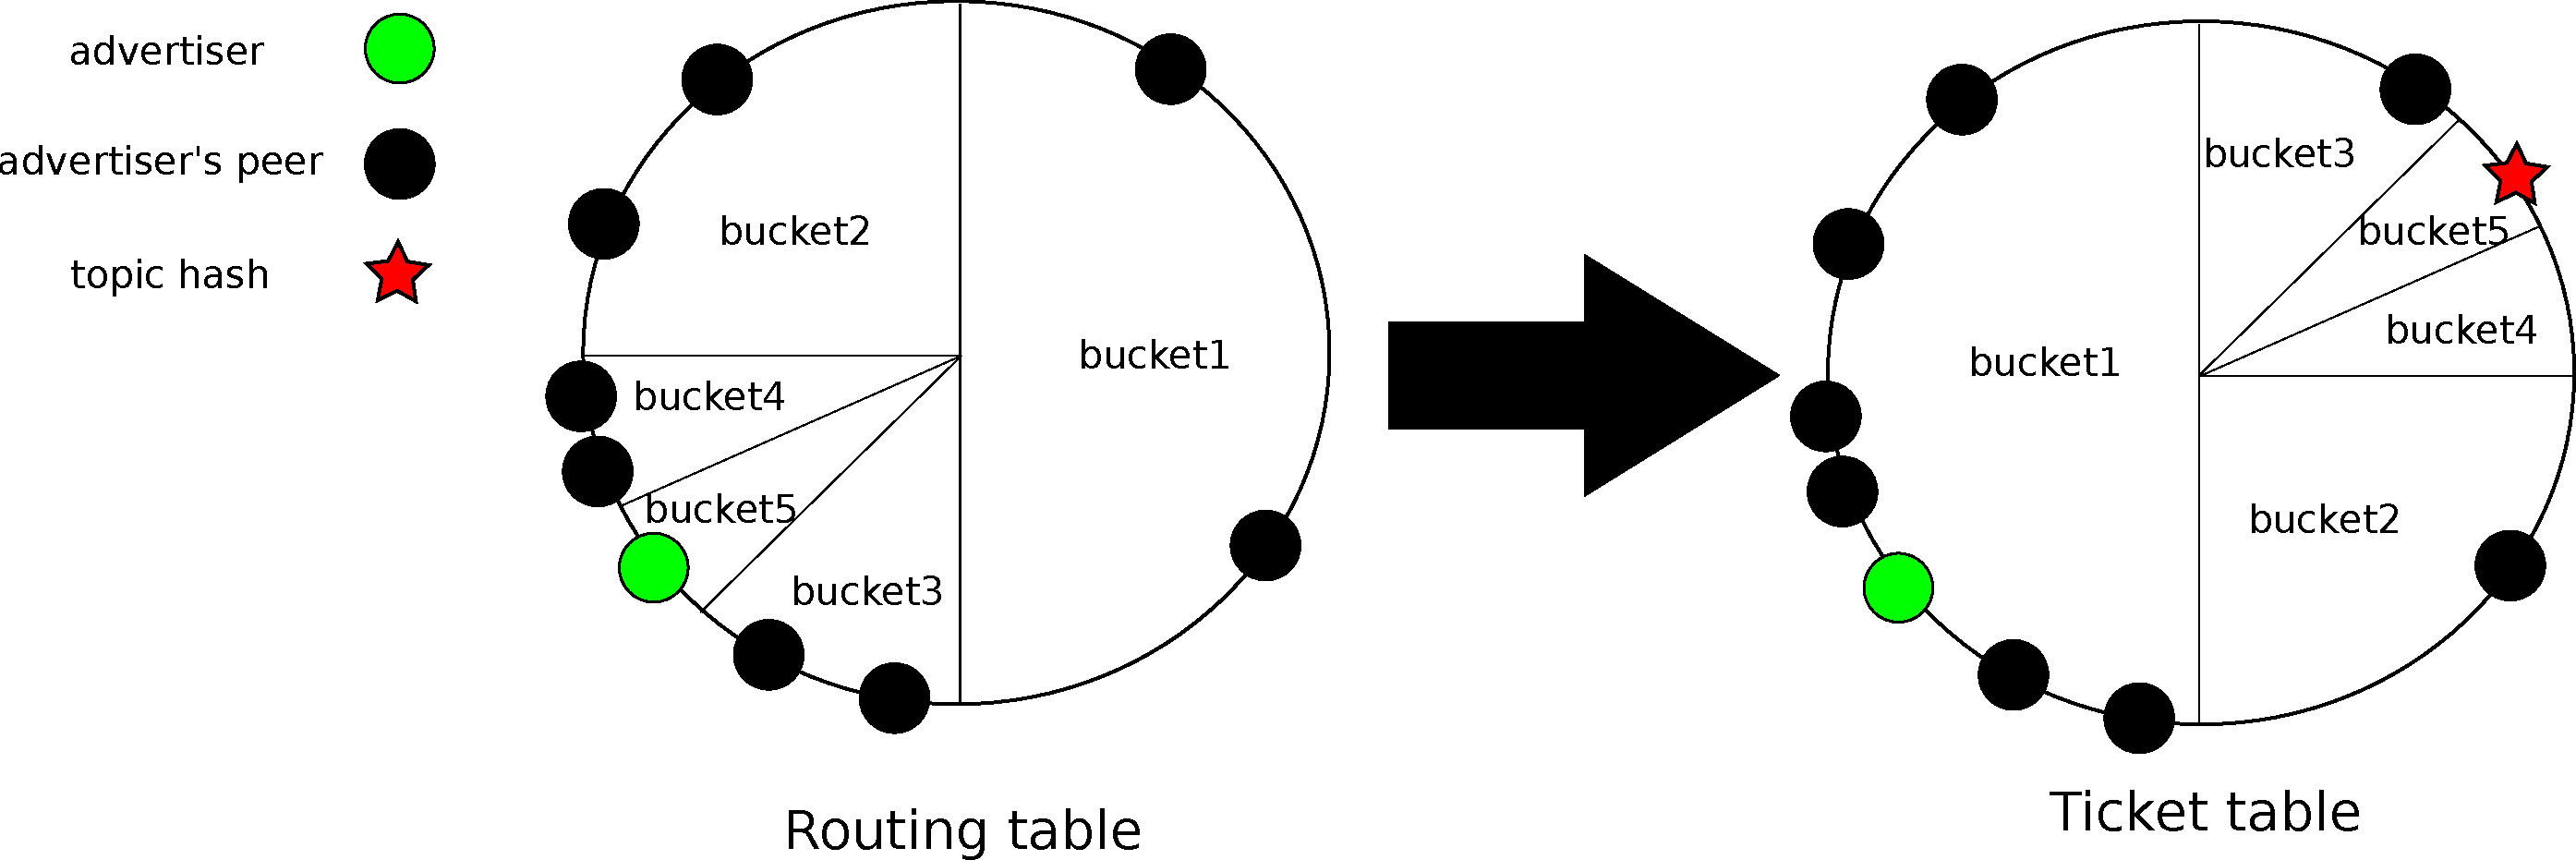
\includegraphics[width=0.5\textwidth]{img/ticket_table}
    \caption{Creation of ticket table from the routing table.}
    \label{fig:ticket_table}
 \end{figure}

\subsection{Lookup}
The lookup operation closely mirrors the registration operation. The searcher starts by creating a \emph{search table}, organized in the same way as the \emph{ticket table} and determined by the topic hash. The searcher then starts the search from the furthest buckets in the search table and progressively moving towards buckets closer to the topic hash. A fixed number of random registrars is contacted for each bucket. Similarly to the registration operation, queried registrars respond with a list of the closest peers to the topic hash the registrars know of, allowing to progressively populate the search table. The search process stops when enough peers were found or when the closest registrar to the topic hash is reached. This approach allow searcher of popular topics to stop the process after a few queries without going all the way towards the topic hash and improves the load balance in the system. On the other hand, searchers of less popular topics are guaranteed to eventually discover all peer subscribed to their topic. 
\fi
